%diagramma
\paragraph{UC-21 Visualizzazione di tutte le postazioni presenti nel sistema}
\begin{itemize}
    \item \textbf{Attori:} amministratore;
    \item \textbf{Descrizione:} un amministratore pu\`{o} visualizzare a video l'insieme delle postazioni registrate in una stanza;
    \item \textbf{Precondizione:} l'amministratore si trova nella pagina di visualizzazione delle stanze registrate nell'applicazione web;
    \item \textbf{Postcondizione:} l'amministratore visualizza tutte le postazioni all'interno della stanza selezionata;
    \item \textbf{Scenario principale:}
    \begin{itemize}
        \item l'amministratore, dall'elenco delle stanze registrate nel sistema, seleziona una stanza desiderata ed accede alla schermata di visualizzazione delle postazioni registrate al suo interno. Da questa schermata, l'amministratore può visualizzare le postazioni per codice identificativo (UC-21.1 Visualizzazione postazione per codice identificativo), visualizzare tutte le postazioni prenotate (UC-21.2 Visualizzazione postazioni prenotate), visualizzare le postazioni occupate (UC-21.3 Visualizzazione postazioni occupate), visualizzare le postazioni libere (UC-21.4 Visualizzazione postazioni libere), visualizzare le postazioni igienizzate (UC-21.5 Visualizzazione postazioni igienizzate), visualizzare le postazioni sporche (UC-21.6 Visualizzazione postazioni sporche), visualizzare le postazioni abilitate(UC-21.7 Visualizzazione postazioni abilitate) ed, infine, visualizzare le postazioni disabilitate (UC-21.8 Visualizzazione postazioni disabilitate). In alternativa, l'amministratore può filtrare le postazioni anche per stanza di appartenenza.
        \item l'amministratore visualizza tutte le postazioni presenti nella stanza precedentemente selezionata.
    \end{itemize}
\end{itemize}

\begin{figure}[H]
    \centering
      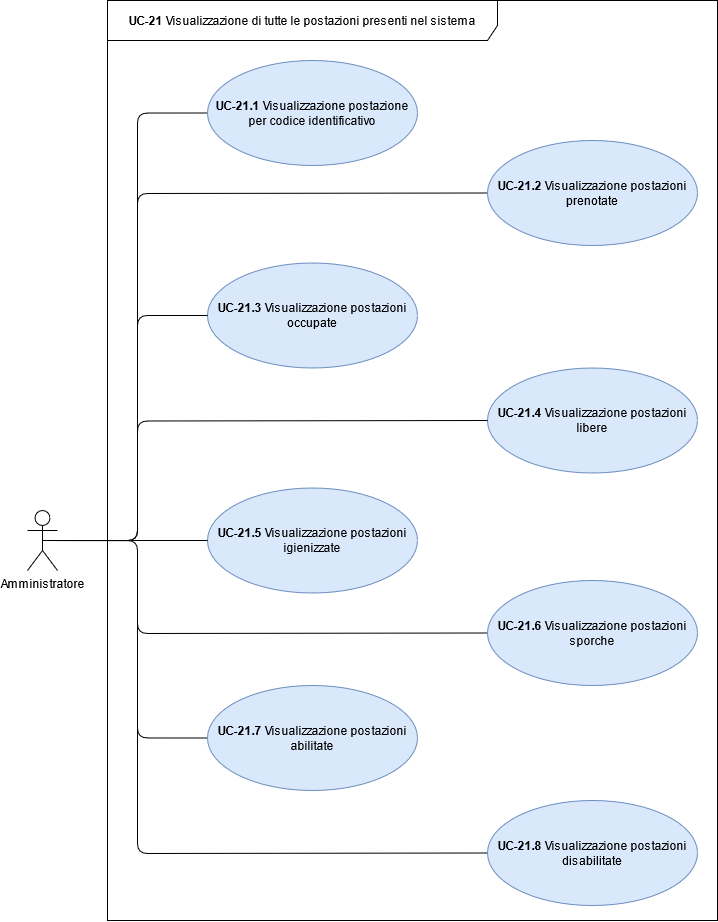
\includegraphics[scale=0.50]{src/CasiDUso/immagini/VisualizzazionePostazioni.png}
    \caption{Diagramma relativo alla visualizzazione di tutte le stanze nel sistema}
\end{figure}

\paragraph{UC-21.1 Visualizzazione postazione per codice identificativo}
\begin{itemize}
    \item \textbf{Attori:} amministratore;
    \item \textbf{Descrizione:} un amministratore pu\`{o} visualizzare una postazione censita nel sistema tramite codice identificativo;
    \item \textbf{Precondizione:} l'amministratore visualizza l'elenco di tutte le postazioni registrate nel sistema;
    \item \textbf{Postcondizione:} l'amministratore ricerca un insieme di postazioni tramite filtro attivo e visualizza la postazione cui codice identificativo è uguale a quello cercato. Se non esiste alcuna postazione avente il codice identificativo inserito dall'amministratore, non verrà visualizzato alcun risultato a video;
    \item \textbf{Scenario principale:}
    \begin{enumerate}
        \item l'amministratore applica il filtro nella lista di postazioni mostrate a video;
        \item una volta applicato il filtro, vengono scremati i risultati non corrispondenti al filtro stesso, e rimarrà a video solamente la postazione registrata nel sistema avente codice identificativo simile a quello cercato dall'amministratore. Nel caso in cui non esista alcuna postazione con criterio corrispondente al filtro, non verrà mostrato a video alcun risultato.
    \end{enumerate}
\end{itemize}


\paragraph{UC-21.2 Visualizzazione postazioni prenotate}
\begin{itemize}
    \item \textbf{Attori:} amministratore;
    \item \textbf{Descrizione:} un amministratore pu\`{o} visualizzare un insieme di postazioni prenotate censite nel sistema;
    \item \textbf{Precondizione:} l'amministratore visualizza l'elenco di tutte le postazioni registrate nel sistema;
    \item \textbf{Postcondizione:} l'amministratore ricerca un insieme di postazioni tramite filtro attivo e visualizza una elenco di postazioni cui stato è prenotato. Se non esiste alcuna postazione prenotata, non verrà visualizzato alcun risultato a video;
    \item \textbf{Scenario principale:}
    \begin{enumerate}
        \item l'amministratore applica il filtro nella lista di postazioni mostrate a video;
        \item una volta applicato il filtro, vengono scremati i risultati non corrispondenti al filtro stesso, e rimarranno a video solamente le postazioni prenotate. Nel caso in cui non esista alcuna postazione con criterio corrispondente al filtro, non verrà mostrato a video alcun risultato.
    \end{enumerate}
\end{itemize}

\paragraph{UC-21.3 Visualizzazione postazioni occupate}
\begin{itemize}
    \item \textbf{Attori:} amministratore;
    \item \textbf{Descrizione:} un amministratore pu\`{o} visualizzare un insieme di postazioni occupate censite nel sistema;
    \item \textbf{Precondizione:} l'amministratore visualizza l'elenco di tutte le postazioni registrate nel sistema;
    \item \textbf{Postcondizione:} l'amministratore ricerca un insieme di postazioni tramite filtro attivo e visualizza una elenco di postazioni cui stato è occupato. Se non esiste alcuna postazione occupata, non verrà visualizzato alcun risultato a video;
    \item \textbf{Scenario principale:}
    \begin{enumerate}
        \item l'amministratore applica il filtro nella lista di postazioni mostrate a video;
        \item una volta applicato il filtro, vengono scremati i risultati non corrispondenti al filtro stesso, e rimarranno a video solamente le postazioni occupate. Nel caso in cui non esista alcuna postazione con criterio corrispondente al filtro, non verrà mostrato a video alcun risultato.
    \end{enumerate}
\end{itemize}

\paragraph{UC-21.4 Visualizzazione postazioni libere}
\begin{itemize}
    \item \textbf{Attori:} amministratore;
    \item \textbf{Descrizione:} un amministratore pu\`{o} visualizzare un insieme di postazioni libere censite nel sistema;
    \item \textbf{Precondizione:} l'amministratore visualizza l'elenco di tutte le postazioni registrate nel sistema;
    \item \textbf{Postcondizione:} l'amministratore ricerca un insieme di postazioni tramite filtro attivo e visualizza una elenco di postazioni cui stato è libero. Se non esiste alcuna postazione libera, non verrà visualizzato alcun risultato a video;
    \item \textbf{Scenario principale:}
    \begin{enumerate}
        \item l'amministratore applica il filtro nella lista di postazioni mostrate a video;
        \item una volta applicato il filtro, vengono scremati i risultati non corrispondenti al filtro stesso, e rimarranno a video solamente le postazioni libere. Nel caso in cui non esista alcuna postazione con criterio corrispondente al filtro, non verrà mostrato a video alcun risultato.
    \end{enumerate}
\end{itemize}

\paragraph{UC-21.5 Visualizzazione postazioni igienizzate}
\begin{itemize}
    \item \textbf{Attori:} amministratore;
    \item \textbf{Descrizione:} un amministratore pu\`{o} visualizzare un insieme di postazioni igienizzate censite nel sistema;
    \item \textbf{Precondizione:} l'amministratore visualizza l'elenco di tutte le postazioni registrate nel sistema;
    \item \textbf{Postcondizione:} l'amministratore ricerca un insieme di postazioni tramite filtro attivo e visualizza una elenco di postazioni cui stato è igienizzato. Se non esiste alcuna postazione igienizzata, non verrà visualizzato alcun risultato a video;
    \item \textbf{Scenario principale:}
    \begin{enumerate}
        \item l'amministratore applica il filtro nella lista di postazioni mostrate a video;
        \item una volta applicato il filtro, vengono scremati i risultati non corrispondenti al filtro stesso, e rimarranno a video solamente le postazioni igienizzate. Nel caso in cui non esista alcuna postazione con criterio corrispondente al filtro, non verrà mostrato a video alcun risultato.
    \end{enumerate}
\end{itemize}

\paragraph{UC-21.6 Visualizzazione postazioni sporche}
\begin{itemize}
    \item \textbf{Attori:} amministratore;
    \item \textbf{Descrizione:} un amministratore pu\`{o} visualizzare un insieme di postazioni sporche censite nel sistema;
    \item \textbf{Precondizione:} l'amministratore visualizza l'elenco di tutte le postazioni registrate nel sistema;
    \item \textbf{Postcondizione:} l'amministratore ricerca un insieme di postazioni tramite filtro attivo e visualizza una elenco di postazioni cui stato è sporco. Se non esiste alcuna postazione sporca, non verrà visualizzato alcun risultato a video;
    \item \textbf{Scenario principale:}
    \begin{enumerate}
        \item l'amministratore applica il filtro nella lista di postazioni mostrate a video;
        \item una volta applicato il filtro, vengono scremati i risultati non corrispondenti al filtro stesso, e rimarranno a video solamente le postazioni sporche. Nel caso in cui non esista alcuna postazione con criterio corrispondente al filtro, non verrà mostrato a video alcun risultato.
    \end{enumerate}
\end{itemize}

\paragraph{UC-21.7 Visualizzazione postazioni abilitate}
\begin{itemize}
    \item \textbf{Attori:} amministratore;
    \item \textbf{Descrizione:} un amministratore pu\`{o} visualizzare un insieme di postazioni abilitate censite nel sistema;
    \item \textbf{Precondizione:} l'amministratore visualizza l'elenco di tutte le postazioni registrate nel sistema;
    \item \textbf{Postcondizione:} l'amministratore ricerca un insieme di postazioni tramite filtro attivo e visualizza una elenco di postazioni cui stato è abilitato. Se non esiste alcuna postazione abilitata, non verrà visualizzato alcun risultato a video;
    \item \textbf{Scenario principale:}
    \begin{enumerate}
        \item l'amministratore applica il filtro nella lista di postazioni mostrate a video;
        \item una volta applicato il filtro, vengono scremati i risultati non corrispondenti al filtro stesso, e rimarranno a video solamente le postazioni abilitate. Nel caso in cui non esista alcuna postazione con criterio corrispondente al filtro, non verrà mostrato a video alcun risultato.
    \end{enumerate}
\end{itemize}

\paragraph{UC-21.8 Visualizzazione postazioni disabilitate}
\begin{itemize}
    \item \textbf{Attori:} amministratore;
    \item \textbf{Descrizione:} un amministratore pu\`{o} visualizzare una insieme di postazioni disabilitate censite nel sistema;
    \item \textbf{Precondizione:} l'amministratore visualizza l'elenco di tutte le postazioni registrate nel sistema;
    \item \textbf{Postcondizione:} l'amministratore ricerca un insieme di postazioni tramite filtro attivo e visualizza una elenco di postazioni cui stato è disabilitato. Se non esiste alcuna postazione disabilitata, non verrà visualizzato alcun risultato a video;
    \item \textbf{Scenario principale:}
    \begin{enumerate}
        \item l'amministratore applica il filtro nella lista di postazioni mostrate a video;
        \item una volta applicato il filtro, vengono scremati i risultati non corrispondenti al filtro stesso, e rimarranno a video solamente le postazioni disabilitate. Nel caso in cui non esista alcuna postazione con criterio corrispondente al filtro, non verrà mostrato a video alcun risultato.
    \end{enumerate}
\end{itemize}
    
\paragraph{UC-22 Visualizzazione informazioni sulla postazione}
\begin{itemize}
    \item \textbf{Attori:} amministratore;
    \item \textbf{Descrizione:} un amministratore pu\`{o} visualizzare a video tutte le informazioni disponibili di una determinata postazione registrata nel sistema;
    \item \textbf{Precondizione:} l'amministratore si trova nella pagina di visualizzazione delle postazioni di una stanza registrate nell'applicazione web;
    \item \textbf{Postcondizione:} l'amministratore visualizza tutti i dettagli della postazione selezionata;
    \item \textbf{Scenario principale:}
    \begin{enumerate}
        \item l'amministratore, dall'elenco delle postazioni registrate nel sistema, seleziona una postazione desiderata ed accede alla schermata di visualizzazione delle informazioni quali codice postazione (UC-22.1 Visualizzazione codice postazione), stato postazione (UC-22.2 Visualizzazione stato della postazione) e stato pulizia della postazione per la postazione scelta (UC-22.3 Visualizzazione stato pulizia della postazione);
        \item l'amministratore visualizza tutte informazioni per la postazione precedentemente selezionata.
    \end{enumerate}
\end{itemize}

\begin{figure}[H]
    \centering
      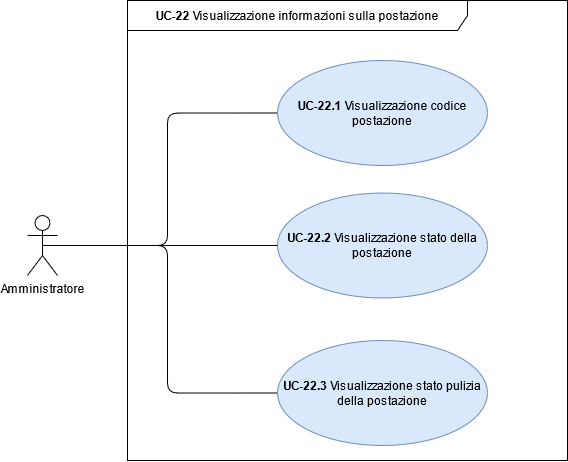
\includegraphics[scale=0.50]{src/CasiDUso/immagini/InformazioniPostazione.png}
    \caption{Diagramma relativo alla visualizzazione delle informazioni di una specifica postazione nel sistema}
\end{figure}

\paragraph{UC-22.1 Visualizzazione codice postazione}
\begin{itemize}
    \item \textbf{Attori:} amministratore;
    \item \textbf{Descrizione:} un amministratore pu\`{o} visualizzare a video il codice identificativo univoco di una postazione precedentemente selezionata;
    \item \textbf{Precondizione:} l'amministratore sta visualizzando a video i dettagli di una postazione selezionata;
    \item \textbf{Postcondizione:} l'amministratore visualizza il codice identificativo della postazione desiderata;
    \item \textbf{Scenario principale:}
    \begin{enumerate}
        \item l'amministratore visualizza a video il codice identificativo univoco della postazione precedentemente selezionata.
    \end{enumerate}
\end{itemize}

\paragraph{UC-22.2 Visualizzazione stato della postazione}
\begin{itemize}
    \item \textbf{Attori:} amministratore;
    \item \textbf{Descrizione:} un amministratore pu\`{o} visualizzare a video lo stato di una postazione all'interno di una stanza precedentemente selezionata;
    \item \textbf{Precondizione:} l'amministratore sta visualizzando a video i dettagli di una postazione selezionata;
    \item \textbf{Postcondizione:} l'amministratore visualizza lo stato della postazione (prenotata, libera o occupata) interna alla stanza selezionata;
    \item \textbf{Scenario principale:}
    \begin{enumerate}
        \item l'amministratore visualizza a video lo stato di una postazione interna alla stanza selezionata.
    \end{enumerate}
\end{itemize}
    

\paragraph{UC-22.3 Visualizzazione stato pulizia della postazione} 
\begin{itemize}
    \item \textbf{Attori:} amministratore;
    \item \textbf{Descrizione:} un amministratore pu\`{o} visualizzare a video lo stato di pulizia di una postazione all'interno della stanza precedentemente selezionata;
    \item \textbf{Precondizione:} l'amministratore sta visualizzando a video i dettagli di una postazione selezionata;
    \item \textbf{Postcondizione:} l'amministratore visualizza lo stato di pulizia della postazione (sporca o igienizzata) interna alla stanza selezionata;
    \item \textbf{Scenario principale:}
    \begin{enumerate}
        \item l'amministratore visualizza a video lo stato di pulizia una postazione interna alla stanza selezionata.
    \end{enumerate}
\end{itemize}

\paragraph{UC-23 Aggiunta di una nuova postazione}
\begin{itemize}
    \item \textbf{Attori:} amministratore;
    \item \textbf{Descrizione:} un amministratore pu\`{o} aggiungere una postazione alla lista di postazioni disponibili all'interno di una stanza. Per inserire una nuova postazione, l'amministrazione prima seleziona la stanza dove inserire la nuova postazione (UC-23.1 Selezione stanza), successivamente, è richiesto l'inserimento del codice identificativo della postazione (UC-23.2 Inserimento codice postazione) ed infine, inserire il codice del tag RFID per associarlo alla postazione appena creata (UC-23.3 Inserimento codice del tag RFID);
    \item \textbf{Precondizione:} l'amministratore si trova nella pagina di gestione delle postazioni nell'applicazione web;
    \item \textbf{Postcondizione:} una nuova postazione \`{e} stata aggiunta alla lista di postazioni disponibili;
    \item \textbf{Scenario principale:}
    \begin{enumerate}
        \item l'amministratore inserisce le informazioni riguardanti la postazione da aggiungere, quali stanza (UC-23.1 Selezione stanza), codice postazione (UC-23.2 Inserimento codice postazione) e codice del tag RFID (UC-23.3 Inserimento codice del tag RFID);
        \item l'amministratore conferma le informazioni inserite e, se corrette, sono salvate nel sistema.
    \end{enumerate}
\end{itemize}

\begin{figure}[H]
    \centering
      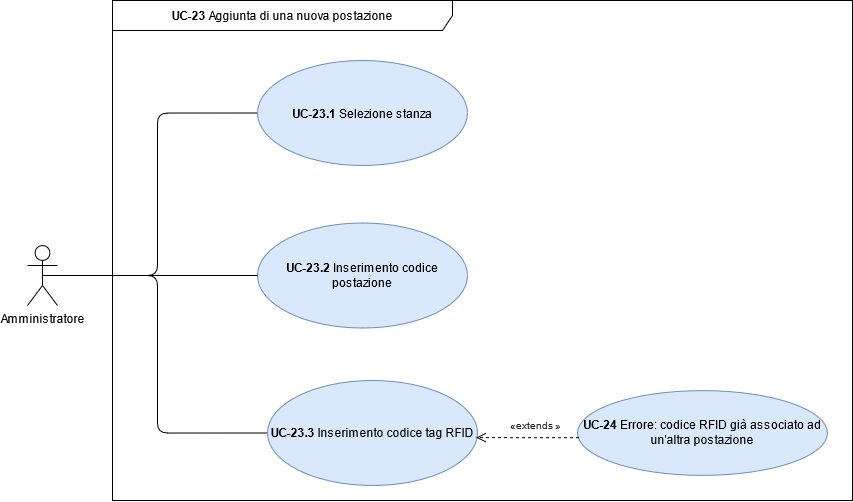
\includegraphics[scale=0.30]{src/CasiDUso/immagini/AggiuntaPostazione.png}
    \caption{Diagramma relativo all'aggiunta di una nuova postazione nel sistema}
\end{figure}

\paragraph{UC-23.1 Selezione stanza}
\begin{itemize}
    \item \textbf{Attori:} amministratore;
    \item \textbf{Descrizione:} un amministratore pu\`{o} selezionare una stanza già censita nel sistema dove inserire una nuova postazione dall'elenco delle stanze nel form di inserimento di una nuova postazione;
    \item \textbf{Precondizione:} l'amministratore sta visualizzando a video il form di inserimento di una nuova postazione;
    \item \textbf{Postcondizione:} l'amministratore ha selezionato correttamente una stanza censita all'interno del sistema;
    \item \textbf{Scenario principale:}
    \begin{enumerate}
        \item l'amministratore seleziona la stanza dall'elenco delle stanze censite dove inserire la nuova postazione.
    \end{enumerate}
\end{itemize}


\paragraph{UC-23.2 Inserimento codice postazione}
\begin{itemize}
	\item \textbf{Attore primario:} amministratore;
	\item \textbf{Descrizione:} l'amministratore inserisce un codice identificativo univoco per contrassegnare la nuova postazione all'interno della stanza selezionata nel form di inserimento di una nuova postazione;
	\item \textbf{Precondizioni:} l'amministratore sta visualizzando a video il form di inserimento di una nuova postazione;
	\item \textbf{Postcondizioni:} l'amministratore inserisce il codice identificativo della postazione con successo;
	\item \textbf{Scenario principale:}
	      \begin{enumerate}
		      \item l'amministratore inserisce il codice identificativo della nuova postazione che si vuole aggiungere;
		      \item il sistema controlla l'univocità del codice inserito. Qualora questa sia rispettata, elaborerà correttamente la richiesta, altrimenti mostrerà a video un messaggio di errore esplicativo (UC-25 Errore: codice postazione non valido)
	      \end{enumerate}
          \begin{itemize}
            \item UC-25 Errore: codice postazione non valido.
        \end{itemize}
\end{itemize}
    

 \paragraph{UC-23.3 Inserimento codice del tag RFID}
 \begin{itemize}
	\item \textbf{Attore primario:} amministratore;
	\item \textbf{Descrizione:} l'amministratore inserisce il codice tag RFID per contrassegnare la nuova postazione all'interno della stanza selezionata nel form di inserimento di una nuova postazione;
	\item \textbf{Precondizioni:} l'amministratore sta visualizzando a video il form di inserimento di una nuova postazione;
	\item \textbf{Postcondizioni:} l'amministratore inserisce il codice del tag RFID della postazione con successo;
	\item \textbf{Scenario principale:}
	      \begin{enumerate}
		      \item l'amministratore inserisce il codice tag RFID della nuova postazione che si vuole aggiungere;
		      \item il sistema controlla l'univocità del codice inserito. Qualora questa sia rispettata, elaborerà correttamente la richiesta, altrimenti mostrerà a video un messaggio di errore esplicativo (UC-24 Errore: codice RFID già associato ad un'altra postazione)
	      \end{enumerate}
	      \item \textbf{Estensioni:}
		\begin{itemize}
		      \item UC-24 Errore: codice RFID già associato ad un'altra postazione.
	      \end{itemize}
\end{itemize}

\paragraph{UC-24 Errore: codice RFID già associato ad un'altra postazione}
    \begin{itemize}
	\item \textbf{Attore primario:} amministratore;
	\item \textbf{Descrizione:} il sistema non permette l'assegnazione di quel codice RFID se esso è già stato utilizzato in un'altra postazione censita. In tal caso viene mostrato un errore a video auto esplicativo;
	\item \textbf{Precondizioni:} l'amministratore ha inserito un codice RFID già associato ad un'altra postazione;
	\item \textbf{Postcondizioni:} il sistema restituisce un messaggio d'errore esplicativo e non completa l'inserimento del codice RFID;
	\item \textbf{Scenario principale:}
	      \begin{enumerate}
	      	      \item l'amministratore invia i dati al sistema;
		      \item il sistema rileva una postazione già censita con lo stesso codice RFID;
		      \item il sistema restituisce un messaggio d'errore esplicativo e non permette di completare l'inserimento del codice RFID relativo alla postazione.
	      \end{enumerate}
\end{itemize}


\paragraph{UC-25 Errore: codice postazione non valido}
\begin{itemize}
	\item \textbf{Attore primario:} amministratore;
	\item \textbf{Descrizione:} l'amministratore inserisce un codice identificativo errato di nuova postazione all'interno della stanza selezionata nel form di inserimento o modifica di una postazione;
	\item \textbf{Precondizioni:} l'amministratore ha inserito un codice identificativo errato relativo ad una postazione;
	\item \textbf{Postcondizioni:} il sistema restituisce un messaggio d'errore esplicativo e non completa l'inserimento del codice della postazione;
	\item \textbf{Scenario principale:}
	      \begin{enumerate}
		      \item il sistema elabora la richiesta ricevuta;
		      \item il sistema restituisce un messaggio d'errore esplicativo che viene visualizzato sullo schermo del dispositivo dell'amministratore e non completa l'inserimento del codice identificativo della postazione.
	      \end{enumerate}
\end {itemize}

\paragraph{UC-25.1 Errore: codice postazione non univoco}
    \begin{itemize}
	\item \textbf{Attore primario:} amministratore;
	\item \textbf{Descrizione:} il sistema non permette l'assegnazione di quel nome se il codice identificativo della nuova postazione è già stato utilizzato. In tal caso viene mostrato un errore a video auto esplicativo;
	\item \textbf{Precondizioni:} l'amministratore ha inserito un codice postazione già censito nel sistema;
	\item \textbf{Postcondizioni:} il sistema restituisce un messaggio d'errore esplicativo e non completa l'inserimento del nuovo codice postazione;
	\item \textbf{Scenario principale:}
	      \begin{enumerate}
	      	      \item l'amministratore invia i dati al sistema;
		      \item il sistema rileva una postazione già censita con lo stesso codice;
		      \item il sistema restituisce un messaggio d'errore esplicativo e non permette di completare l'inserimento del codice identificativo relativo alla nuova postazione.
	      \end{enumerate}
\end{itemize}
    
\paragraph{UC-25.2 Errore: il codice postazione contiene caratteri non validi}
\begin{itemize}
	\item \textbf{Attore primario:} amministratore;
	\item \textbf{Descrizione:} l'amministratore ha provato ad inserire un nuovo codice identificativo ma l'assegnazione non è andata a buon fine poiché il codice inserito contiene dei caratteri speciali che non rispettano i criteri di inserimento;
	\item \textbf{Precondizioni:} l'amministratore ha inserito un codice postazione che contiene dei caratteri non validi durante l'assegnazione del codice alla nuova postazione;
	\item \textbf{Postcondizioni:} il sistema restituisce un messaggio d'errore esplicativo e non completa l'inserimento del nuovo codice postazione;
	\item \textbf{Scenario principale:}
	      \begin{enumerate}
		      \item il sistema rileva dei caratteri non validi all'interno del codice della postazione;
		      \item il sistema restituisce un messaggio d'errore esplicativo e non permette di completare l'inserimento del codice identificativo relativo alla nuova postazione.
	      \end{enumerate}
\end{itemize}


\paragraph{UC-26 Modifica dati di una postazione}
\begin{itemize}
    \item \textbf{Attori:} amministratore;
    \item \textbf{Descrizione:} un amministratore pu\`{o} modificare i dati di una postazione già esistente modificando, nello specifico, il codice della postazione e/o il codice RFID;
    \item \textbf{Precondizione:} l'amministratore si trova nella pagina di gestione delle postazioni nell'applicazione web;
    \item \textbf{Postcondizione:} l'amministratore ha modificato con successo i dati relativi ad una postazione esistente;
    \item \textbf{Scenario principale:}
    \begin{itemize}
        \item l'amministratore seleziona, dalla lista delle postazioni, la postazione da modificare;
        \item l'amministratore modifica il codice postazione (UC-26.1 Modifica codice postazione) e/o il codice RFID (UC-26.2 Modifica codice tag RFID);
        \item l'amministratore conferma le informazioni inserite e, se corrette, sono salvate nel sistema.
    \end{itemize}
\end{itemize}

\begin{figure}[H]
    \centering
      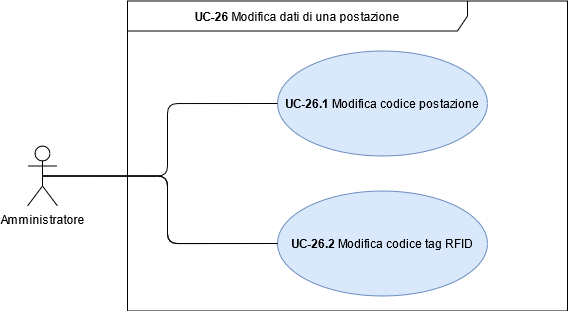
\includegraphics[scale=0.35]{src/CasiDUso/immagini/ModificaPostazione.png}
    \caption{Diagramma relativo alla modifica dei dati di una postazione nel sistema}
\end{figure}


\paragraph{UC-26.1 Modifica codice postazione}
  \begin{itemize}
	\item \textbf{Attore primario:} amministratore;
	\item \textbf{Descrizione:} l'amministratore vuole modificare il codice di una postazione già censita nel sistema;
	\item \textbf{Precondizioni:} l'amministratore ha selezionato la funzionalità di modifica del codice identificativo per una postazione già censita nel sistema;
	\item \textbf{Postcondizioni:} l'amministratore ha modificato con successo il codice di una postazione;
	\item \textbf{Scenario principale:}
	      \begin{enumerate}
		      \item l'amministratore seleziona l'apposita funzionalità di modifica del codice identificativo della postazione precedentemente selezionata;
		      \item il sistema controlla l'univocità del codice inserito. Qualora questa sia rispettata, elaborerà correttamente la richiesta, altrimenti mostrerà a video un messaggio di errore esplicativo (UC-25 Errore: codice postazione non valido).
	      \end{enumerate}
	\item \textbf{Estensioni:}
		\begin{itemize}
		      \item UC-25 Errore: codice postazione non valido.
	      \end{itemize}
\end{itemize}

    
\paragraph{UC-26.2 Modifica codice tag RFID}
\begin{itemize}
    \item \textbf{Attori:} amministratore;
    \item \textbf{Descrizione:} un amministratore pu\`{o} modificare il tag RFID di una postazione già censita nel sistema;
    \item \textbf{Precondizione:} l'amministratore ha selezionato la funzionalità di modifica del codice tag RFID per una postazione già censita nel sistema;
    \item \textbf{Postcondizione:} l'amministratore ha modificato con successo il codice tag RFID di una postazione;
    \item \textbf{Scenario principale:}
    \begin{itemize}
        \item l'amministratore seleziona l'apposita funzionalità di modifica del codice tag RFID della postazione precedentemente selezionata;
        \item il sistema controlla l'univocità del codice inserito. Qualora questa sia rispettata, elaborerà correttamente la richiesta, altrimenti mostrerà a video un messaggio di errore esplicativo (UC-24 Errore: codice RFID già associato ad un'altra postazione).
    \end{itemize}
    \item \textbf{Estensioni:}
		\begin{itemize}
		      \item UC-24 Errore: codice RFID già associato ad un'altra postazione.
	      \end{itemize}
\end{itemize}

 
\paragraph{UC-27 Rimozione di una postazione dal sistema}
\begin{itemize}
    \item \textbf{Attori:} amministratore;
    \item \textbf{Descrizione:} un amministratore pu\`{o} rimuovere una postazione dalla lista di postazioni disponibili all'interno di una stanza. Per rimuovere una postazione, l'amministratore accede alla schermata di dettaglio della postazione che si desidera rimuovere e, successivamente, l'amministratore selezionerà la funzione di rimozione della postazione selezionata. Una volta rimossa la postazione, tutte le prenotazioni vengono annullate;
    \item \textbf{Precondizione:} l'amministratore si trova nella pagina di gestione delle postazioni nell'applicazione web;
    \item \textbf{Postcondizione:} una postazione \`{e} stata rimossa dalla lista di postazioni disponibili, e le prenotazioni attive per la prenotazione rimossa vengono annullate;
    \item \textbf{Scenario principale:}
    \begin{itemize}
        \item l'amministratore, dall'elenco delle postazioni registrate nel sistema, seleziona la postazione desiderata ed accede alla schermata di visualizzazione delle informazioni proprie della postazione selezionata;
        \item l'amministratore seleziona la funzionalità di rimozione della postazione selezionata;
        \item l'amministratore conferma la volontà di rimozione della postazione e questa viene rimossa dal sistema. Tutte le prenotazioni relativa alla postazione in oggetto vengono cancellate.
    \end{itemize}
\end{itemize}

\paragraph{UC-28 Disabilitazione di una postazione}
\begin{itemize}
    \item \textbf{Attori:} amministratore;
    \item \textbf{Descrizione:} un amministratore pu\`{o} disabilitare una postazione dalla lista di postazioni disponibili all'interno di una stanza. Per disabilitare una postazione, l'amministratore accede alla schermata di dettaglio della postazione che si desidera disabilitare e, successivamente, l'amministratore selezionerà la funzione di disabilitazione della postazione selezionata. Una volta disabilitata la postazione, tutte le prenotazioni vengono annullate;
    \item \textbf{Precondizione:} l'amministratore si trova nella pagina di gestione delle postazioni nell'applicazione web;
    \item \textbf{Postcondizione:} una postazione \`{e} stata disabilitata con successo, e le prenotazioni attive per la prenotazione rimossa vengono annullate;
    \item \textbf{Scenario principale:}
    \begin{itemize}
        \item l'amministratore, dall'elenco delle postazioni registrate nel sistema, seleziona la postazione desiderata ed accede alla schermata di visualizzazione delle informazioni proprie della postazione selezionata;
        \item l'amministratore seleziona la funzionalità di disabilitazione della postazione selezionata;
        \item l'amministratore conferma la volontà di disabilitare la postazione e questa viene disabilitata dal sistema. Tutte le prenotazioni relativa alla postazione in oggetto vengono cancellate.
    \end{itemize}
\end{itemize}

\paragraph{UC-29 Riabilitazione di una postazione precedentemente disabilitata}
\begin{itemize}
    \item \textbf{Attori:} amministratore;
    \item \textbf{Descrizione:} un amministratore pu\`{o} ri-abilitare una postazione precedentemente segnata come disabilitata all'interno di una stanza. Per ri-abilitare una postazione, l'amministratore accede alla schermata di dettaglio della postazione che si desidera ri-abilitare e, successivamente, l'amministratore selezionerà la funzione di ri-abilitazione della postazione selezionata. Una volta ri-abilitata la postazione, questa torna ad essere fruibile e prenotabile dagli utenti;
    \item \textbf{Precondizione:} l'amministratore si trova nella pagina di gestione delle postazioni nell'applicazione web;
    \item \textbf{Postcondizione:} una postazione \`{e} stata ri-abilitata con successo, quindi prenotabile e servibile nuovamente;
    \item \textbf{Scenario principale:}
    \begin{itemize}
        \item l'amministratore, dall'elenco delle postazioni registrate nel sistema, seleziona la postazione desiderata ed accede alla schermata di visualizzazione delle informazioni proprie della postazione selezionata;
        \item l'amministratore seleziona la funzionalità di ri-abilitazione della postazione selezionata;
        \item l'amministratore conferma la volontà di ri-abilitare la postazione e questa viene abilitata dal sistema. Una postazione abilitata è di nuovo fruibile dagli utenti e prenotabile.
    \end{itemize}
\end{itemize}
